% !TEX root = ../main.tex
\section{Introduction}

This is demo text for testing the writing setup. It is not part of the proposal. Each section
lives in its own file under \texttt{sections/}, and \texttt{main.tex} pulls them together, so
one section can be rewritten without touching the others.

Citations use IEEE style: a single source appears as~\cite{lamport1994latex}, and two together
as~\cite{lamport1994latex,knuth1984texbook}. Figures are numbered and referenced the same way:
Fig.~\ref{fig:sandbox} shows the arm in the planned sandbox.

% Source: https://github.com/vertical-cloud-lab/robot-arms/blob/bdb25d3/lab-models/renders/sandbox_scene.png
% (branch claude/issue-199-20260915-0846). AI-generated render; arm from AgileX's CAD model.
\begin{figure}[htbp]
  \centering
  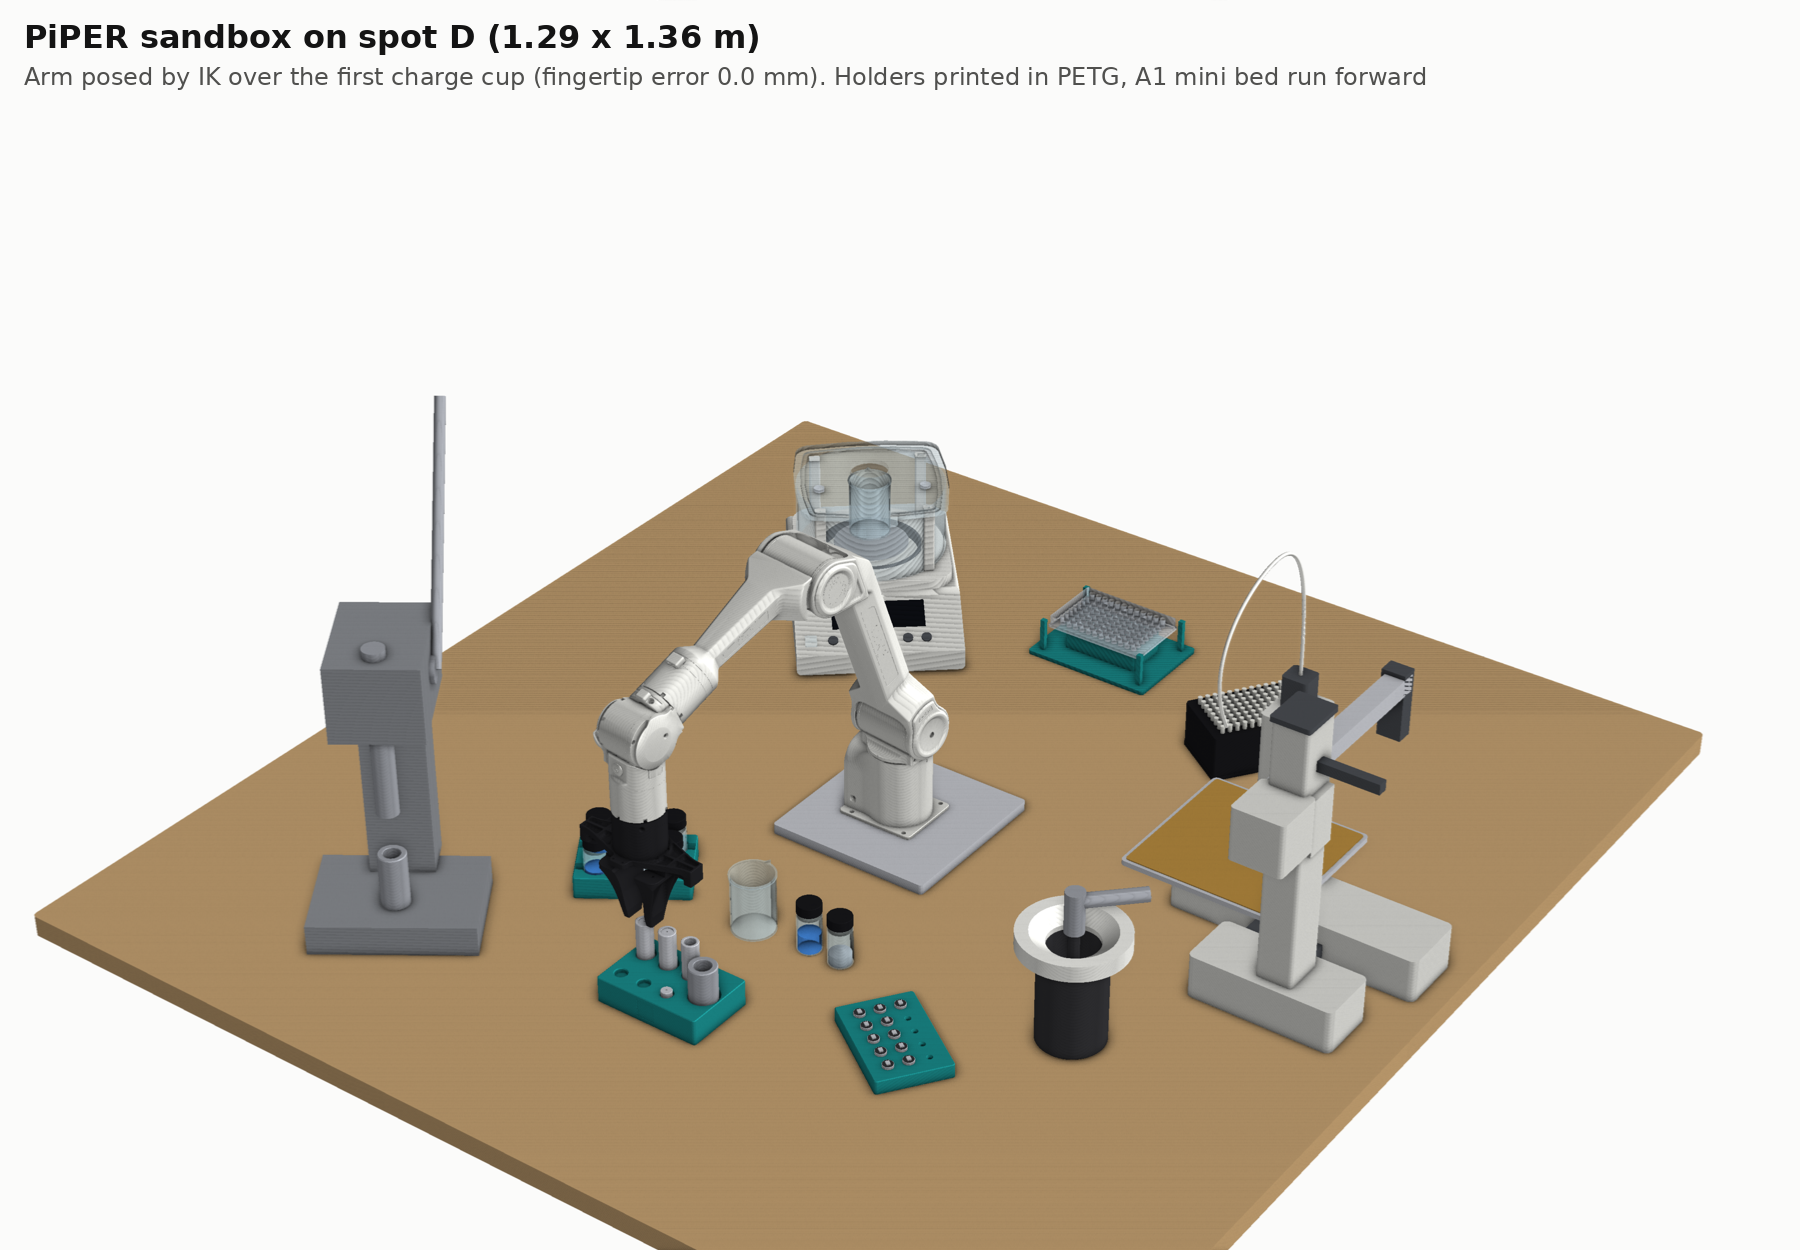
\includegraphics[width=0.9\linewidth]{sandbox_scene}
  \caption{Rendered layout of the PiPER sandbox (1.29\,m $\times$ 1.36\,m), with the arm posed
    over a charge cup among the lab equipment and printed labware holders it is meant to serve.
    The arm is rendered from AgileX Robotics' CAD model.}
  \label{fig:sandbox}
\end{figure}
